\documentclass[12pt,a4paper,oneside]{report}
% =================================================================================================================
% Ulster University research degree thesis: unofficial LaTeX template.
% Layout follows the Doctoral College "Format of Thesis" guidance and the "Guidance for printing of theses for
% research degrees" (check the current versions before submission; links in README.md):
%   A4 portrait; sans-serif font (Helvetica or Arial) 12 pt; line spacing 1.5; an additional line space after each
%   paragraph; page numbers in the top outer corner, roman for the preliminary pages; binding margin at least 40 mm,
%   other margins at least 20 mm; title page with title, author, faculty, degree, month and year and the word-count
%   statement; abstract of at most 300 words; contents with lists of figures and tables; abbreviations;
%   acknowledgements; captions below figures and titles above tables; UK English; Harvard referencing.
% =================================================================================================================
\usepackage[british]{babel}
\usepackage[utf8]{inputenc}
\usepackage[T1]{fontenc}
\usepackage[scaled=1]{helvet}\renewcommand{\familydefault}{\sfdefault}      % Helvetica (sans-serif)
\usepackage[left=40mm,right=25mm,top=25mm,bottom=25mm,headheight=15pt]{geometry}   % binding margin 40 mm
\usepackage{setspace}\onehalfspacing                                          % 1.5 line spacing
\usepackage[parfill]{parskip}                                                 % space after each paragraph
\usepackage{fancyhdr}                                                          % page number top outer corner
\pagestyle{fancy}\fancyhf{}\fancyhead[R]{\thepage}\renewcommand{\headrulewidth}{0pt}
\fancypagestyle{plain}{\fancyhf{}\fancyhead[R]{\thepage}\renewcommand{\headrulewidth}{0pt}}
\usepackage{amsmath,amssymb}
\usepackage{graphicx}
\usepackage{booktabs,tabularx,longtable,array,multirow}
\usepackage{adjustbox}
\usepackage{xcolor}
\usepackage{enumitem}
\usepackage[section]{placeins}
\usepackage[font=small,labelfont=bf]{caption}
\usepackage[round,authoryear]{natbib}
\bibpunct{(}{)}{;}{a}{}{,}                                                    % Harvard: (Author Year), no comma
\usepackage[hidelinks]{hyperref}
\hypersetup{colorlinks=true,linkcolor={blue!45!black},citecolor={blue!45!black},urlcolor={blue!70!black},bookmarksnumbered=true}
\usepackage[capitalise,noabbrev]{cleveref}
\usepackage[acronym,nonumberlist,toc]{glossaries}\makeglossaries

\graphicspath{{figures/}}
\newcolumntype{Y}{>{\raggedright\arraybackslash}X}
\newcolumntype{P}[1]{>{\raggedright\arraybackslash}p{#1}}
% ---------------------------------------------------------------------------------------------------------------
% Your details: the only file you need to edit before writing.
% ---------------------------------------------------------------------------------------------------------------
\newcommand{\ThesisTitle}{Title of the thesis:\\ and its sub-title}
\newcommand{\ThesisAuthor}{Full Name}
% Faculty, as on the Ulster University title page, for example:
%   Faculty of Life and Health Sciences | Faculty of Arts, Humanities and Social Sciences |
%   Faculty of Computing, Engineering and the Built Environment | Ulster University Business School
\newcommand{\ThesisFaculty}{Faculty of Life and Health Sciences}
\newcommand{\ThesisDegree}{Doctor of Philosophy}
\newcommand{\SubmissionMonthYear}{Month Year}
\newcommand{\ThesisKeywords}{keyword one, keyword two}

% Key of abbreviations (Ulster: a key is required; write a term in full at first use with the abbreviation in brackets).
% \newacronym{label}{SHORT}{long form}; every abbreviation defined here is listed (\glsaddall in main.tex).
\newacronym{gis}{GIS}{geographic information system}
\newacronym{prisma}{PRISMA}{Preferred Reporting Items for Systematic Reviews and Meta-Analyses}

\glsaddall                                                                    % list every abbreviation defined

\begin{document}
\pagenumbering{roman}
\begin{titlepage}
\centering\onehalfspacing
{\Large\bfseries \ThesisTitle\par}
\vspace{2cm}
{\large \ThesisAuthor\par}
\vspace{1.5cm}
\ThesisFaculty{} of Ulster University\par
\vspace{1cm}
Thesis submitted for the degree of \ThesisDegree\par
\vspace{1cm}
\SubmissionMonthYear\par
\vfill
I confirm that the word count of this thesis is less than 100,000 words excluding the title page, contents,
acknowledgements, summary or abstract, abbreviations, footnotes, diagrams, maps, illustrations, tables, appendices,
and references or bibliography.\par
\end{titlepage}

\chapter*{Abstract}\addcontentsline{toc}{chapter}{Abstract}
% Ulster: at most 300 words. A synopsis: the nature and scope of the work, its contribution to knowledge, a brief
% statement of the methods, an outline of the main divisions or arguments, and a summary of the conclusions.
Write the abstract here.

\tableofcontents
\listoffigures
\listoftables
\printglossary[type=\acronymtype,title=Abbreviations]
\chapter*{Acknowledgements}\addcontentsline{toc}{chapter}{Acknowledgements}
% Ulster: acknowledge any assistance received; in collaborative work, state your own contribution; state any part of
% the work previously submitted for another degree.
Write the acknowledgements here.

\chapter*{Declaration on the use of generative artificial intelligence}\label{ch:ai-declaration}
\addcontentsline{toc}{chapter}{Declaration on the use of generative artificial intelligence}
% Declaration on the use of generative AI. Follow the Ulster University Doctoral College guidance on the use of
% generative AI tools (Research Studies Guide) and agree the use with your supervisory team. Delete this page if no
% generative AI was used and your guidance does not require a statement.
This declaration follows the Ulster University Doctoral College guidance on the use of generative artificial
intelligence (AI) tools. The use described here was agreed with the supervisory team on [date].

\textbf{Tools.} [Name and version of each tool, and the period of use.]

\textbf{Purposes.} [For example: code assistance; checking references; language editing; drafting of specified
sections, which were checked and revised by the candidate.]

\textbf{Not delegated.} [For example: the research questions, design, analysis, interpretation and conclusions.]

\textbf{Responsibility.} The candidate takes full responsibility for the content of this thesis.

\clearpage
\pagenumbering{arabic}

\chapter{Introduction}\label{ch:introduction}

\section{Background}\label{sec:background}
Text with a citation in Harvard style \citep{page2021}, or naming the authors, as \citet{roberts2017} show.
Cross-references are written with \verb|\cref|: \cref{ch:methods}, \cref{tab:example}, \cref{fig:example} and
\cref{app:supplement}.

\section{Aim, objectives and research questions}\label{sec:aims}
\begin{enumerate}[label=O\arabic*.]
  \item First objective.
  \item Second objective.
\end{enumerate}

\section{Structure of the thesis}\label{sec:structure}
\Cref{ch:literature} reviews the literature, \cref{ch:methods} describes the methods, \cref{ch:results} presents the
results, \cref{ch:discussion} discusses them and \cref{ch:conclusions} concludes.

\chapter{Literature review}\label{ch:literature}
\section{Review method}\label{sec:review-method}
For a systematic review, report the methods following PRISMA 2020 \citep{page2021}.

\section{Data}\label{sec:data}
Equations are numbered by chapter:
\begin{equation}
  \bar{x} = \frac{1}{n}\sum_{i=1}^{n} x_i .
\end{equation}

\section{Validation}\label{sec:validation}
Describe how results are validated, for example with spatially separated test data \citep{roberts2017}.

\section{Main results}\label{sec:main-results}
Tables have their title above (Ulster), figures their caption below.

\begin{table}[htbp]
  \centering\small
  \caption{An example table (title above the table).}\label{tab:example}
  \begin{tabular}{lrr}
    \toprule
    Group & Mean & SD \\
    \midrule
    A & 1.20 & 0.30 \\
    B & 1.45 & 0.28 \\
    \bottomrule
  \end{tabular}
\end{table}

\begin{figure}[htbp]
  \centering
  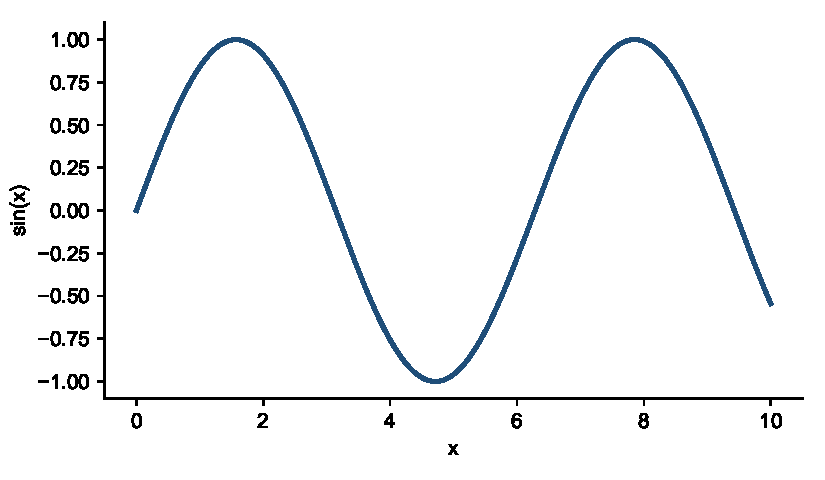
\includegraphics[width=0.7\linewidth]{thesis-example-figure}
  \caption{An example figure (caption below the figure).}\label{fig:example}
\end{figure}

\section{Principal findings}\label{sec:findings}
Discuss the findings.
\section{Limitations}\label{sec:limitations}
State the limitations.

Conclude, and give recommendations and future work.


\cleardoublepage\phantomsection\addcontentsline{toc}{chapter}{\bibname}
\bibliographystyle{agsm}
\bibliography{references}

\appendix
\chapter{Supplementary material}\crefalias{chapter}{appendix}\label{app:supplement}
% Appendices come before the references (Ulster order). Use \chapter for each appendix in main.tex.
Supplementary tables, code descriptions or data registers.


% Ulster order: main text, appendices, then references
\bibliographystyle{agsm}
\bibliography{references}

\end{document}
